% !TEX TS-program = pdflatex
% !TEX encoding = UTF-8 Unicode
% !TEX ROOT = main.tex

\newcounter{zahl}
% \newcommand{\altstadtkarte}{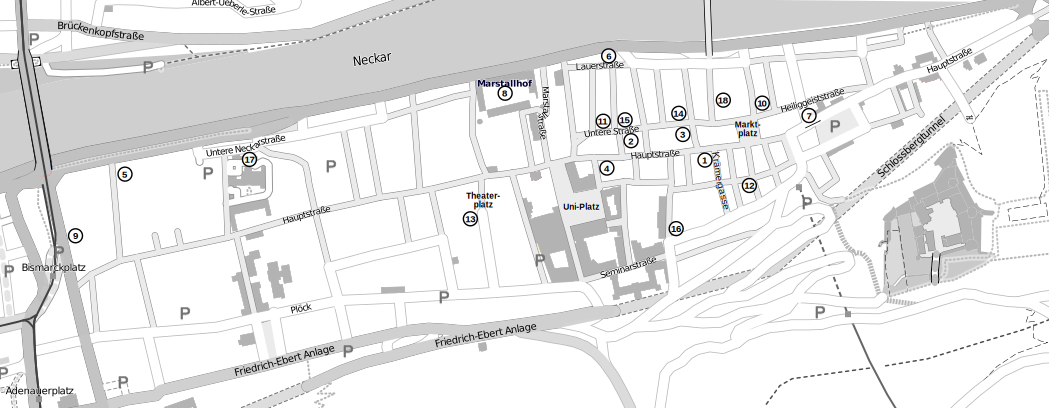
\includegraphics[width=\textwidth, trim=10mm 0mm 80mm 0mm, clip]{media/altstadtkarte}} % Vektorgrafik einbinden
\newcommand{\place}[4]{\item[(\stepcounter{zahl}\thezahl) #1](#2)\\ #3\\\emph{Preis:} #4}

\section{Bars, Kneipen \& Diskotheken}
\subsection*{In der Altstadt:}
Preis: $\star$ teuer, $\star\ \star$ noch teurer, $\star\ \star\ \star$ extrem teuer


\begin{description}

%    \place{Alfredo}{Untere Straße}{Wirklich sehr leckere Pizza, der Chef sorgt für den echt italienischen Flair.}{$\star$}

    \place{Cave 54}{Krämergasse 1}{(Deutschlands ältester) Jazzkeller. Kostet am Wochen\-ende Eintritt, hat dafür allerdings noch nach 3 Uhr geöffnet.}{$\star\ \star$}

%    \place{Coyote}{Hauptstraße}{Einer der Orte, um eine Kneipentour durch die Altstadt starten zu lassen. Weizenbier, Cocktails und Shots sind brauchbar und brauchen nicht ewig.}{$\star\ \star$}

    \place{Destille}{Untere Straße}{Große Auswahl an Shots. Kultiger Laden mit ständig wechselnder Dekoration.}{$\star\ \star$}

    \place{Eckstein}{am Fischmarkt 3}{Abgefahrene Kneipe. Je nach Wochentag ändert sich das Programm. Es gibt jedoch immer einen Kicker und reichlich Platz. Drei Mal wöchentlich Zaubershows.}{$\star\ \star$}

    \place{Hard Rock Cafe}{Hauptstraße 142}{Montags Bier für \EUR{1}, ab 18 Uhr Cocktails für \EUR{4}. Musik wie man es erwartet, durchgehend Rock.}{$\star$}

%    \place{Havanna}{Neckarstaden 24}{Cocktailbar mit Möglichkeit zum Salsa tanzen.}{$\star\ \star\ \star$}

    \place{Hemmingways}{Fahrtgasse 1}{Hier lässt es sich das gesamte Jahr draußen sitzen, dank warmen Decken und Heizstrahlern. Außerdem kann man wunderbar den Neckar beobachten.}{$\star\ \star$}

    \place{Karls}{Lauerstraße 7-9}{Kneipe mit Billardtisch und Dartscheibe. Gut um sich voll\/laufen zu lassen oder einfach nur zu versacken.}{$\star\ \star$}

    \place{Karlstorbahnhof}{Am Karlstor\,/\,S-Bahnhof Altstadt}{Richtig gute Diskothek (Nicht nur; im Gebäude gibts auch Theater, Lesungen etc. -- viel Kultur) mit sehr variabler Musik. Was zum tanzen und weniger zum trinken, denn die Preise können sich meistens sehen lassen, genauso der Eintritt}{$\star\ \star\ \star$}

    \place{Marstall}{Marstallhof}{Keine typische Kneipe, vielmehr Mensa mit Bier. Trotzdem gut geeignet sich zu treffen, zum Vorglühen und entscheiden, wo die weitere Party ihren Anfang nehmen soll.}{$\star$}

%    \place{Maxbar}{Marktplatz 5}{Hier gibt es des öfteren Live-Musik}{$\star\ \star$}

    \place{Medoc}{Bismarckplatz}{Cafe Restaurant das für ca. \EUR{5} wechselnde Mittagsgerichte anbietet. Man kann draußen sitzen und den Betrieb auf dem Bismarckplatz beobachten.}{$\star\ \star$}

    \place{Mels}{Heiliggeiststr. 1}{Gewölbekeller in dem seit Jahren die selbe Musik läuft, aber zumindest weiß man dann, was einen erwartet. Haben unter der Woche immer sehr gute Spezialangebote z.B. Dienstags 123-Party (Bier \EUR{1}, Weizen 2, Cocktails 3).}{$\star\ \star$}

    \place{Mohr}{Untere Straße}{Hoher MedizinerInnen Anteil, Einlass erst ab 20 Jahren und spät abends meist so voll, dass man gar nicht mehr rein kommt. Drinnen wird dafür allerdings auf den Tischen getanzt.}{$\star\ \star$}

    \place{Orange}{Ingrimmstraße 26a}{Eine Kneipe wie ein Wohnzimmer. Eng aber gemütlich. Bietet sehr leckeres Bier aus Tschechien an, ist aber leider eher verraucht. Es gibt sogar Brettspiele.}{$\star\ \star$}

%    \place{Palmbräugasse}{Untere Straße}{Hier gibts das selbstgebraute Palmbräu. Palmen gehören zwar nicht typisch zu Heidelberg, aber die Schnitzel in der Palmbräugasse.}{$\star\ \star$}

    \place{Regie}{Theaterplatz}{Riesenauswahl an Cocktails, die nach Filmen benannt und meist recht schick dekoriert sind. Cooles Specials- und Aktionensystem und leckere Flammkuchen}{$\star\ \star\ \star$}

    \place{Reichsapfel}{Untere Straße}{Sehr geräumig. Moderner Vorderbereich und urigere Atmosphäre im hinteren Teil, welcher über den Innenhof zugänglich ist. Dort findet man oft Platz wenn sonst alles voll ist.}{$\star\ \star$}

    \place{Sonderbar}{Untere Straße}{Jede nur erdenkliche Form von Absinth, auch viel guten Rum und Whisky. Immer ordentlich was auf die Ohren (Hard \& Heavy). Keine Angst vor dem Wirt, einfach nicht auf den Mund gefallen sein. Oft sehr voll und vollgeräuchert.}{$\star\ \star$}

    \place{Tangente}{Kettengasse 23}{Hoher JuristInnenanteil und teils ältere Menschen. Türsteher und Gesichtskontrolle, dafür aber kein Eintritt. Hier kann man bis in die frühen Morgenstunden tanzen, man sollte allerdings keine Platzangst haben.}{$\star\ \star$}

    \place{Vater Rhein}{Untere Neckarstraße 20}{Legendär für seine \EUR{1,90}-Spaghetti bis halb drei. Hier lässt sich der Abend gemütlich ausklingen.}{$\star$}

	\place{Vetters}{Steingasse 9}{Nicht zum Bleiben, aber für die Maß to go. Gibts da für \EUR{3}, schmeckt hervorragend. Ansonsten gutbürgerliche Küche und älteres Klientel}{$\star\ \star$}

\end{description}

% trim=l b r t
\hspace*{-6mm}
% \altstadtkarte
  \todo{altstadtkarte aus media/altstadtkarte.svg einbinden}
    \todo{Boho vllt noch einfügen}

%%%%%%%%%
\subsection{In den Stadtteilen:}
\begin{description}

    \place{Bar 133}{Wohnheim INF 133}{Wohnheimsbar, eigentlich nur für Bewohner der 1xx Wohnheime. Mittwochs und sonntags geöffnet mit gutem Angebot, günstigen Cocktails und Tischkicker. Immer wieder für einen Absturz gut.}{$\star$}

	\place{Comabar}{Comenius-Haus}{Bar des Comenius-Hauses direkt am Bunsengymnasium. Dienstags und Donnerstags geöffnet, super Team, günstige Cocktails, Kicker und Tischtennisplatte vorhanden. Definitiv empfehlenswert.}{$\star$}

%    \place{Breidenbach Studios}{Hebelstraße 18}{Absoluter Hipster-Laden: Ehemalige Gasflaschenhandlung, die zu einem Künstlerhaus und Coworking-Space umgebaut wurde. Hier finden immer wieder großartige Partys statt.}{$\star\ \star\ \star$}

    \place{Cappuchino}{Bergheimer Straße 8}{Hippe Mischung von Kaffeehaus mit lautem Elektro.}{$\star\ \star$}

    \place{Gilberts Goldener Adler}{Handschuhsheimer Landstraße 96}{Ist eigentlich ein Restaurant, hat im Sommer aber auch einen netten Biergarten. Die Portionen sind groß und lecker. Stammlokal einiger Matheprofs.}{$\star\ \star$}

    \place{Halle 02}{Bahnstadt}{Electrofreunde werden hier ihren Spaß haben, es gibt aber auch viele Mainstream Partys. Meistens sind diese auch recht voll und es herrscht gute Stimmung. Ab und zu spielen auch bekanntere Bands.}{$\star\ \star$}

    \place{O'Reilly's}{Brückenkopfstraße 1}{Irish Pub mit Karaoke.}{$\star\ \star\ \star$}

    \place{P11}{Am Römerkreis}{Nettes Café, dass Abends bis etwa eins Barbetrieb hat. Trotz der Nähe zum Römerkreis angenehme Atmosphäre. Geile Tapete!}{$\star\ \star$}

    \place{Villa Nachttanz}{Im Klingenbühl 6}{Alternativer Kulturverein -- rechnet mit allem außer Mainstream. Sehr günstig, mit Lagerfeuer im Garten. Lohnt sich jedes mal.}{$\star$}

    \place{Ziegler}{Bergheimer Straße 1}{Kneipe mit Disco, welche allerdings Eintritt kostet und auch sonst recht hohe Preise hat. Oft auch Live Musik}{$\star\ \star\ \star$}

    \place{Zwitscherstube}{Blumenstraße 25}{Urige Kneipe mit Alt, Kölsch und original Underberggürtel. Hier kommen vor allem Fußballfans auf ihre Kosten. Wenn kein Fußball läuft kann man super Skat spielen.}{$\star$}


\end{description}
